\part{El desconocido NoSQL} 
\chapter{Introducci\'on a NoSQL}

\section{Definici\'on}

NoSQL o "No solamente SQL" ({\bf Not Only SQL}) es un t\'ermino acu\~nado por Carlo Strozzi en 1998 y nuevamente retomado por Eric Evans en 2009 y se refiere a un conjuto de bases de datos que se diferencian en gran parte de las bases de datos convencionales, en caracter\'isticas tanto de uso como de implementaci\'on; estos tipos de bases de datos no usan SQL o al menos no como lenguaje predeterminado para realizar las consultas. Las bases de datos NoSQL (desde ahora "no relacionales"), no soportan totalmente {\bf ACID} \footnote{'ACID: Atomicidad, Coherencia, Aislamiento y Durabilidad'}, esto lo explica el teorema del profesor Eric Brewer, Teorema CAP (2000):

\begin{quote}
Es imposible para un sistema distribuido garantizar simultáneamente las siguientes tres características:

	\begin{itemize}
		\item Consistency (Consistencia): todos los nodos ven la misma data al mismo tiempo.
		\item Availability (Disponibilidad): una garantía de que todos los requerimientos recibirán una respuesta de que el requerimiento fue exitoso o fallido.
		\item Partition Tolerance (Tolerancia a la Partición): el sistema continúa operando a pesar de la pérdida arbitraria de mensajes, o la falla de parte del sistema.
	\end{itemize}
\end{quote}

En primera instancia es una desventaja, pero gracias a esto permite que los motores de bases de datos no relacionales escalen f\'acilmente de manera horizontal. 

El lenguaje SQL no es un lenguaje predominante entre los distintos tipos de bases de datos no relacionales, por lo general cada motor tiene su propio lenguaje de consultas. Cabe destacar que la informaci\'on no se almacena con un esquema fijo (\textbf{pero si usando almacenamiento estructurado}), aun que si existe un esquema que el DBA\footnote{'Database Administrator - Administrador de base de datos'} o el desarrollador propone con anterioridad de manera virtual, es decir, no se crea en el motor antes de utilizar la base de datos sino al almacenar el primer valor.

\section{Tipos de bases de datos no relacionales}

En el mundo de las bases de datos no relacionales nos encontramos con distintos modelos o tipos, que se desempe\~nan mejor en algunos ambientes espec\'ificos; esas distintas facetas no se ven en las base de datos relacionales. En este libro se expondr\'an los tipos m\'as comunes.

\subsection{Bases de datos orientadas a documentos}

Las bases de datos orientadas a documentos o tambi\'en denominadas como {\bf Bases de datos documental}, trabajan bajo el marco de la definici\'on de un \textit{"Documento"}, donde cada motor que usa esta definici\'on difiere en los detalles, pero la mayor\'ia concuerda en como se almacena la informaci\'on con alg\'un formato est\'andar. Los formatos m\'as utilizados por los motores m\'as populares son: {\bf JSON y BSON}. Se podr\'ia  considerar este tipo como el m\'as utilizada en la actualidad.

Cada documento, es muy similar a un registro en una base de datos relacional, donde se puede observar un esquema parecido mas no r\'igido. Dos documentos no tienen porque tener un esquema igual, aunque sean de una misma colecci\'on de datos.

\begin{figure}[!ht]
    \centering
    \begin{lstlisting}
    {
	    _id: 1,
	    nombre: "MongoDB",
	    url: "http://www.mongodb.org",
	    tipo: "Documental"
    }
    \end{lstlisting}
    \caption[Bases de datos documental]{Ejemplo de documento.}
\end{figure}

Este ejemplo demuestra la sencillez de un documento, se observa un modelo al estilo \textit{\textbf{clave : valor}}. Una analog\'ia con las bases de datos relacionales ser\'ia: Clave = Campo y Valor = Dato del campo, hasta all\'i queda la analog\'ia.

\subsection{Bases de datos orientadas a clave/valor}

Este tipo de bases de datos es muy similar a las bases de datos documental en el concepto de guardar la informaci\'on con el modelo clave:valor, la diferencia radica en que un documento se almacena en una clave; esta definici\'on puede parecer algo abstracta. Esto se explica mejor con un ejemplo.

El siguiente ejemplo utiliza el documento de la secci\'on anterior:

\begin{figure}[!ht]
    \centering
    \begin{lstlisting}
    mongodb => {
	    _id: 1,
	    nombre: "MongoDB",
	    url: "http://www.mongodb.org",
	    tipo: "Documental"
    }
    \end{lstlisting}
    \caption[Bases de datos clave/valor]{Ejemplo de un documento en una clave.}
\end{figure}

La clave en este caso es 'mongodb' y su contenido es el mismo documento de la secci\'on anterior. Esto hace que var\'ie la forma de recuperar la informaci\'on con respecto a las bases de datos basadas en documentos.

Algun muy interesante de este tipo es que permite ser utilizado junto bases de datos orientadas a documentos, lo que origina motores h\'ibridos.

\subsection{Bases de datos orientadas a grafos}

\begin{figure}[!h]
    \centering
    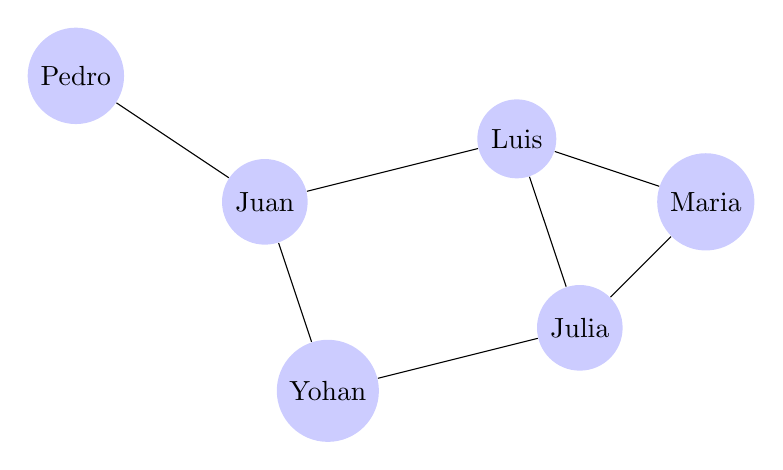
\begin{tikzpicture}
         [scale=.8,auto=left,every node/.style={circle,fill=blue!20}]
         \node (nPedro) at (1,10) {Pedro};
         \node (nJuan) at (4,8)  {Juan};
         \node (nLuis) at (8,9)  {Luis};
         \node (nMaria) at (11,8) {Maria};
         \node (nJulia) at (9,6)  {Julia};
         \node (nYohan) at (5,5)  {Yohan};

         \foreach \from/\to in {nPedro/nJuan,nJuan/nLuis,nLuis/nMaria,nMaria/nJulia,nJulia/nLuis,nJulia/nYohan,nYohan/nJuan}
             \draw (\from) -- (\to);

     \end{tikzpicture}
     \caption[Bases de datos en grafo]{Ejemplo de un gr\'afo con relaciones de conocidos.}
\end{figure}

Este tipo difiere completamente a los tipos antes mencionados, y trata la informaci\'on de una manera peculiar usando \textbf{grafos}\footnote{Grafo: es un conjunto de objetos llamados nodos unidos por enlaces denotados aristas, que permiten representar relaciones binarias entre elementos de un conjunto.} y \textbf{teor\'ia de grafos}. Cada nodo solo debe contener una sola columna, por lo tanto se debe normalizar completamente las bases de datos. Y como la definici\'on de grafos indica, las relaciones solo pueden ser binarias, es decir, un nodo puede solo usar una relaci\'on para entrar en contacto con otro nodo y no m\'as de uno.

Las ventajas de este tipo de bases de datos van enfocadas a la integridad de los datos, cualquier cambio en un nodo o relaci\'on solo afecta localmente.

\section{Sistema de gesti\'on de bases de datos (SGBD)}

Jorge Sánchez Asenjo (2005) define SGBD\footnote{En ingl\'es DBMS: Data Base Management System} como:

\begin{quote}
Un sistema gestor de bases de datos o SGBD es el software que permite a los usuarios procesar, describir, administrar y recuperar los datos almacenados en una base de datos. 
\end{quote}

Un tipo de base de datos no sirve de nada sino tiene un sistema que lo gestione, a menos que desees crear un SGBD. En NoSQL hay una basta gama de SGBD, y la mayor\'ia est\'an bajo licencia de c\'odigo libre, permitiendo as\'i usar, estudiar, modificar y redistribuir sin problema alguno con respecto a algunos motores de bases de datos relacionales con licencias privativas.

\section{Lista de SGBD NoSQL}

\subsection*{Bases de datos documental}

\begin{itemize}
\item MongoDB (Lanzamiento: 2009 / Licencia: GNU AGPL v3.0)
\item CouchDB (Lanzamiento: 2005 / Licencia: Apache License 2.0)
\item Raven DB (Lanzamiento: 2010 / Licencia: GNU AGPL v3.0)
\end{itemize}

\subsection*{Bases de datos clave/valor}

\begin{itemize}
\item Apache Cassandra (Lanzamiento: 2008 / Licencia: Apache License 2.0)
\item Riak (Lanzamiento: 2009 / Licencia: Apache License 2.0)
\item Redis (Lanzamiento: 2009 / Licencia: BSD)
\end{itemize}

\subsection*{Bases de datos en grafos}

\begin{itemize}
\item Neo4j (Lanzamiento: 2009 / Licencia: GNU AGPL v3.0)
\item Dex (Lanzamiento: 2008 / Licencia: Comercial)
\item Sones GraphDB (Lanzamiento: 2012 / Licencia: GNU AGPL v3.0 y comercial)
\end{itemize}

\section{¿Por qu\'e NoSQL?}

En esta \'epoca donde se generan cantidades enormes de datos menos estructurados, las bases de datos relacionales empiezan a mostrar deficiencias, en almacenamiento u operaciones; siendo esta una de las principales razones de impulsar el uso de bases de datos no relacionales. Muchas personas se quejan del movimiento NoSQL, m\'as que todo por una resistencia al cambio que por los "contras" de este tipo de bases de datos; en la actualidad gestionar una cantidad de datos gigantesca no es tan sencillo si piensas en estructuras, esto da pie al "BigData". Otra de las razones relevantes es la arquitectura, que permite escalar horizontalmente de manera sencilla sin tantos problemas de rendimiento. \textbf{En cap\'itulos posteriores veremos que es escalamiento horizontal}.

\section{Casos de Usos}

